\documentclass{standalone}
\usepackage{tikz}
\usetikzlibrary{automata, positioning, arrows}

\begin{document}

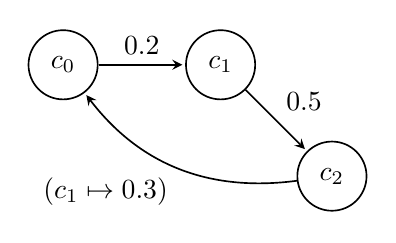
\begin{tikzpicture}[
    > = stealth, % arrow head style
    shorten > = 1pt, % don't touch arrow head to node
    auto,
    node distance = 2cm, % distance between nodes
    semithick % line style
]

% Define nodes
\node[state] (c0) {$c_0$};
\node[state] (c1) [right of=c0] {$c_1$};
\node[state] (c2) [below right of=c1] {$c_2$};

% Draw edges with labels
\path[->] (c0) edge node {0.2} (c1);
\path[->] (c1) edge node {0.5} (c2);
\path[->] (c2) edge[bend left] node {$(c_1 \mapsto 0.3)$} (c0);

\end{tikzpicture}

\end{document}